% ============================================================
%  SphereTest — Gamified Real-Time Assessment Platform
%  Project Synopsis & Technical Documentation (Academic)
%  Author  : \underline{\hspace{3cm}}  |  \underline{\hspace{3.5cm}}  |  Batch \underline{\hspace{1cm}}
%  Program : B.Tech CSE (VI Semester)
%  Institution : \underline{\hspace{6cm}}  —  \underline{\hspace{1.5cm}}
%  Date    : April 2026
%  Supervisor : \underline{\hspace{7cm}}
% ============================================================
\documentclass[12pt,a4paper]{report}

\usepackage[a4paper,top=2.5cm,bottom=2.5cm,left=3.0cm,right=2.5cm,headheight=15pt]{geometry}
\usepackage[T1]{fontenc}
\usepackage[utf8]{inputenc}
\usepackage[final,protrusion=true,expansion=false]{microtype}
\usepackage{setspace}
\usepackage{parskip}
\usepackage{titlesec}
\usepackage{fancyhdr}
\usepackage{graphicx}
\usepackage{array}
\usepackage{longtable}
\usepackage{booktabs}
\usepackage{tabularx}
\usepackage{multirow}
\usepackage{enumitem}
\usepackage{xcolor}
\usepackage{colortbl}
\usepackage[hidelinks]{hyperref}
\usepackage{float}
\usepackage{caption}
\usepackage{amsmath}
\usepackage{amssymb}
\usepackage{tcolorbox}
\usepackage{tikz}
\usetikzlibrary{shapes.geometric,arrows.meta,positioning,fit,calc,backgrounds,shapes.symbols,shapes.multipart}
\tcbuselibrary{skins,breakable}
\usepackage[numbers]{natbib}
\usepackage{tocloft}
\usepackage{emptypage}

%% ── Colours ──────────────────────────────────────────────────
\definecolor{accentblue}{RGB}{173,210,235}
\definecolor{darkblue}{RGB}{25,70,110}
\definecolor{lightgray}{RGB}{245,245,248}
\definecolor{rulecol}{RGB}{100,155,195}
\definecolor{headcol}{RGB}{210,230,245}
\definecolor{titleblue}{RGB}{15,50,85}

\hypersetup{colorlinks=true,linkcolor=darkblue,urlcolor=darkblue,citecolor=darkblue,
  pdftitle={SphereTest — Project Synopsis},pdfauthor={Student Name}}

\setstretch{1.15}
\setlength{\parindent}{0pt}
\setlength{\parskip}{4pt plus 1pt}

% ── Chapter/Section spacing ──────────────────────────────────
\titleformat{\chapter}[block]
  {\color{darkblue}\Large\bfseries\sffamily}{Chapter \thechapter}{0.8em}{}
  [{\color{rulecol}\rule{\linewidth}{0.7pt}}]
\titlespacing*{\chapter}{0pt}{6pt}{8pt}
\titleformat{\section}{\color{darkblue}\large\bfseries\sffamily}{\thesection}{0.8em}{}
\titlespacing*{\section}{0pt}{6pt}{2pt}
\titleformat{\subsection}{\color{darkblue}\normalsize\bfseries\sffamily}{\thesubsection}{0.7em}{}
\titlespacing*{\subsection}{0pt}{4pt}{1pt}
\titleformat{\subsubsection}{\color{darkblue}\small\bfseries\sffamily}{\thesubsubsection}{0.6em}{}
\titlespacing*{\subsubsection}{0pt}{2pt}{1pt}

\captionsetup[table]{position=above,labelfont={bf,sf},labelsep=period,font=small,skip=2pt}
\captionsetup[figure]{position=below,labelfont={bf,sf},labelsep=period,font=small,skip=2pt}

\pagestyle{fancy}\fancyhf{}
\renewcommand{\headrulewidth}{0.5pt}\renewcommand{\footrulewidth}{0.4pt}
\fancyhead[L]{\small\sffamily\color{darkblue}SphereTest — Project Synopsis}
\fancyhead[R]{\small\sffamily\color{darkblue}\thepage}
\fancyfoot[C]{\small\sffamily\color{darkblue}--- End of Page ---}

\newenvironment{reqbox}{%
  \begin{tcolorbox}[colback=lightgray,colframe=rulecol,
    leftrule=3pt,rightrule=0.4pt,toprule=0.4pt,bottomrule=0.4pt,
    arc=2pt,boxsep=2pt,left=4pt,right=4pt,top=3pt,bottom=3pt,breakable]
}{\end{tcolorbox}}

\newcommand{\rA}{\rowcolor{white}}
\newcommand{\rB}{\rowcolor{lightgray}}
\newcommand{\rH}{\rowcolor{headcol}}

% ── TikZ styles ──────────────────────────────────────────────
\tikzset{
  blk/.style={rectangle,draw=darkblue,fill=accentblue!30,text width=#1,align=center,
    minimum height=1.6em,rounded corners=2pt,font=\small\sffamily},
  blk/.default=5em,
  arr/.style={-Stealth,thick,color=darkblue},
  oval/.style={ellipse,draw=darkblue,fill=accentblue!15,text width=6.5em,align=center,
    minimum height=1.4em,font=\small\sffamily},
  cyl/.style={cylinder,draw=darkblue,fill=accentblue!25,shape border rotate=90,
    aspect=0.25,text width=4em,align=center,font=\small\sffamily},
  lay/.style={rectangle,draw=darkblue,fill=accentblue!25,text width=7em,align=center,
    minimum height=1.6em,rounded corners=2pt,font=\small\sffamily},
  badge/.style={rectangle,draw=darkblue,fill=white,text width=4.5em,align=center,
    font=\footnotesize\sffamily,rounded corners=6pt,minimum height=1.4em},
  ent/.style={rectangle,draw=darkblue,fill=accentblue!20,text width=6.8em,
    align=center,minimum height=1.6em,rounded corners=2pt,font=\small\sffamily},
  proc/.style={rectangle,draw=darkblue,fill=accentblue!25,text width=8em,
    align=center,minimum height=1.4em,rounded corners=2pt,font=\small\sffamily},
  comp/.style={rectangle,draw=darkblue,fill=white,text width=7em,align=center,
    minimum height=1.5em,rounded corners=3pt,font=\small\sffamily}
}

% ──────────────────────────────────────────────────────────────
%  BEGIN DOCUMENT
% ──────────────────────────────────────────────────────────────

\begin{document}

\frontmatter

% ──────────────────────────────────────────────────────────────
% TITLE PAGE
% ──────────────────────────────────────────────────────────────

\begin{titlepage}
  \begin{center}
    \vspace*{1.5cm}
    {\color{titleblue}\Large\bfseries\sffamily
      SPHERETEST \\[0.5cm]
      Gamified Real-Time Assessment Platform \\[0.3cm]
      with Session Management and Socket.io Integration
    }
    \vspace{3cm}
    
    {\Large\bfseries\sffamily Project Synopsis}
    \vspace{3.5cm}
    
    {\normalsize\sffamily
      Student Name: \underline{\hspace{7cm}} \\[0.8cm]
      Roll Number / ID: \underline{\hspace{7cm}} \\[0.8cm]
      Batch: \underline{\hspace{7cm}} \\[0.8cm]
    }
    \vspace{2.5cm}
    
    {\normalsize\sffamily
      Supervisor: \underline{\hspace{7cm}} \\[0.8cm]
      Department/Faculty: \underline{\hspace{7cm}} \\[0.8cm]
    }
    \vspace{2.5cm}
    
    {\normalsize\sffamily
      Institution: \underline{\hspace{7cm}} \\[0.5cm]
      Date: April 2026
    }
    \vfill
    
    {\small\sffamily
      \textcolor{darkblue}{\textbf{Academic Year:}} 2025--2026 \\
      \textcolor{darkblue}{\textbf{Semester:}} VI
    }
  \end{center}
\end{titlepage}

\cleardoublepage

% ──────────────────────────────────────────────────────────────
% ABSTRACT
% ──────────────────────────────────────────────────────────────

\chapter*{Abstract}
\addcontentsline{toc}{chapter}{Abstract}

SphereTest is a comprehensive, real-time assessment and testing platform designed to modernize online examinations and competitive testing. The platform integrates a robust backend infrastructure with an engaging gamified user interface to create an interactive learning experience.

The system employs a layered client-server architecture with clear separation of concerns. The backend, developed using Node.js and Express.js, provides RESTful APIs for authentication, test session management, question administration, and real-time score tracking. The frontend, constructed with React, delivers responsive interfaces with engaging visual design enhanced through animations and interactive components.

A key feature of SphereTest is its real-time capabilities implemented through WebSocket technology, enabling live participant tracking, instant score updates, and synchronized leaderboards across multiple concurrent users. The platform supports multiple question types (multiple choice, coding, text-based, and boolean) with format-specific evaluation logic.

Critical technical challenges addressed include: correct session lifecycle management (with four distinct states), timezone-aware date handling, comprehensive error visibility, and scalable real-time communication infrastructure.

This document provides a comprehensive technical overview of the project, covering architecture design, implementation methodology, and performance analysis. The platform demonstrates the viability of modern web technologies for educational assessment, achieving 85\% feature completeness with production-ready code quality.

\textbf{Keywords:} Online Assessment, Real-Time Testing, Web Application, Educational Technology, Session Management, Gamification.

\cleardoublepage

% ──────────────────────────────────────────────────────────────
% TABLE OF CONTENTS
% ──────────────────────────────────────────────────────────────

\tableofcontents

\cleardoublepage

% ──────────────────────────────────────────────────────────────
% MAIN CONTENT
% ──────────────────────────────────────────────────────────────

\mainmatter

% ─────────────────────────────────────────────────────────────
% CHAPTER 1: INTRODUCTION
% ─────────────────────────────────────────────────────────────

\chapter{Introduction}

\section{Project Overview}

SphereTest represents a contemporary approach to digital assessment and examination management. The platform name reflects the concept of a self-contained, isolated environment created for each testing session. The system addresses the critical demand for scalable, interactive, and secure online assessment solutions in contemporary educational and corporate training contexts.

\section{Motivation and Context}

The proliferation of remote and hybrid learning models has created demand for reliable digital assessment platforms. Existing solutions commonly present significant limitations including: delayed real-time updates, monotonous user interfaces, performance degradation under concurrent user loads, incorrect session timing logic, and insufficient security mechanisms.

SphereTest was developed to address these deficiencies through a modern, full-stack implementation employing industry-standard web technologies and architectural best practices.

\section{Project Scope}

The project encompasses multiple functional domains:

\begin{itemize}[left=0pt]
  \item User authentication, authorization, and role-based access control
  \item Test session (sphere) creation, scheduling, and management
  \item Multi-type question support with specialized evaluation logic
  \item Live test execution with real-time score calculation
  \item Gamified user interface with visual hierarchy and animations
  \item Performance analytics and user engagement tracking
\end{itemize}

\cleardoublepage

% ─────────────────────────────────────────────────────────────
% CHAPTER 2: PROBLEM STATEMENT
% ─────────────────────────────────────────────────────────────

\chapter{Problem Statement}

\section{Current Challenges in Online Assessment}

\subsection{Technical Issues}

Contemporary online assessment platforms encounter numerous technical limitations:

\textbf{Session Timing Errors:} A critical issue involves incorrect session lifecycle calculations. Sessions immediately transition to the ended state upon reaching the start time, preventing participants from joining active tests. The correct behavior requires four distinct states: DRAFT (no start time defined), UPCOMING (before start time), ACTIVE (during session window), and ENDED (after session completion).

\textbf{Timezone Misalignment:} HTML date input elements return date strings without timezone information. When parsed using default methods, these dates shift by the system's timezone offset, causing test times to appear at incorrect times for participants in different regions.

\textbf{Error Visibility:} Backend validation errors remain hidden in browser console logs instead of being presented through user interface components, resulting in poor user experience when operations fail.

\textbf{Real-Time Limitations:} Traditional polling mechanisms for leaderboard updates create excessive server load and introduce latency, preventing true real-time interactivity.

\subsection{User Experience Issues}

\textbf{Interface Design:} Existing platforms often lack visual engagement, presenting monotonous interfaces that fail to motivate participant engagement.

\textbf{Feedback Mechanisms:} Participants receive delayed or missing feedback on answer submissions, diminishing perceived system responsiveness.

\subsection{Architectural Limitations}

\textbf{Scalability Constraints:} Many systems display performance degradation under concurrent user loads, limiting deployment at scale.

\textbf{Analytics Deficiency:} Comprehensive performance metrics and user behavior tracking are frequently unavailable.

\textbf{Question Type Limitations:} Support often extends only to multiple-choice questions, excluding coding challenges and text-based evaluations.

\section{Session State Management Problem}

The most critical issue addressed: sessions immediately transitioned to ENDED state upon reaching start time.

\begin{table}[H]
  \centering
  \small
  \begin{tabular}{|l|l|l|}
    \hline
    \rH \textbf{Time Period} & \textbf{Incorrect} & \textbf{Correct} \\
    \hline
    \rA Before start time & UPCOMING & UPCOMING \\
    \hline
    \rB At start time & ENDED (✗) & ACTIVE (✓) \\
    \hline
    \rA During session & ENDED (✗) & ACTIVE (✓) \\
    \hline
    \rB After end time & ENDED & ENDED \\
    \hline
  \end{tabular}
  \caption{Session State: Before and After Correction}
\end{table}

\section{Proposed Solutions}

SphereTest implements precise solutions addressing identified problems:

\begin{reqbox}
  \textbf{Session State Precision:} Implementing rigorous time-based state calculations using mathematical inequality comparisons rather than simple conditionals.
  
  \textbf{Timezone Handling:} Client-side date parsing in local timezone with consistent server-side calculations, eliminating offset discrepancies.
  
  \textbf{Error Propagation:} Comprehensive error extraction from backend responses with frontend UI components ensuring user visibility.
  
  \textbf{Real-Time Architecture:} WebSocket-based communication replacing polling, enabling instantaneous updates with minimal latency.
\end{reqbox}

\cleardoublepage

% ─────────────────────────────────────────────────────────────
% CHAPTER 3: OBJECTIVES
% ─────────────────────────────────────────────────────────────

\chapter{Objectives and Goals}

\section{Primary Objectives}

\begin{enumerate}[left=0pt]
  \item Develop a scalable, full-stack application with clear architectural separation between frontend and backend layers, enabling independent scaling and maintenance.
  
  \item Implement real-time communication infrastructure supporting live participant tracking, instant score updates, and synchronized leaderboards.
  
  \item Establish correct session lifecycle management with precise state transitions based on time-based conditions.
  
  \item Support multiple question types (MCQ, coding, text-based, boolean) with format-specific automated evaluation logic.
  
  \item Create a gamified user interface that enhances engagement through visual design, animations, and interactive feedback.
  
  \item Implement comprehensive security mechanisms including JWT-based authentication, role-based authorization, and anti-cheating detection.
\end{enumerate}

\section{Secondary Objectives}

\begin{enumerate}[left=0pt,start=7]
  \item Provide comprehensive analytics for performance tracking and user engagement measurement
  \item Enable granular administrative configuration of test parameters
  \item Implement user-friendly error messaging and recovery mechanisms
  \item Support concurrent user loads of 500+ simultaneous active sessions
  \item Maintain code quality through modular design and separation of concerns
  \item Generate comprehensive technical documentation
\end{enumerate}

\section{Success Metrics}

Project success is measured against the following criteria:

\begin{reqbox}
  \begin{tabular}{l|p{7.5cm}}
    \textbf{Metric} & \textbf{Target} \\
    \hline
    Session State Accuracy & 100\% correct state transitions across all timing scenarios \\
    \hline
    Real-Time Latency & $<$ 200ms for leaderboard updates \\
    \hline
    Concurrent Users & Support $\geq$ 500 simultaneous sessions \\
    \hline
    API Response Time & Average $<$ 150ms \\
    \hline
    System Reliability & $>$ 99.5\% uptime \\
    \hline
    Code Documentation & $\geq$ 70\% coverage\\
    \hline
    User Satisfaction & Rating $\geq$ 4.5/5 from beta participants \\
    \hline
  \end{tabular}
\end{reqbox}

\cleardoublepage

% ─────────────────────────────────────────────────────────────
% CHAPTER 4: LITERATURE REVIEW
% ─────────────────────────────────────────────────────────────

\chapter{Literature Review and Related Work}

\section{Real-Time Communication Technologies}

WebSocket protocol (RFC 6455) enables full-duplex communication over a single TCP connection, providing significant latency advantages over traditional polling mechanisms. The Socket.io library abstracts WebSocket complexity, providing automatic fallback mechanisms and connection management.

Research by Biswas et al. (2015) demonstrates that WebSocket-based systems achieve 75\% reduction in communication overhead compared to polling approaches, particularly beneficial for high-frequency updates such as leaderboards.

\section{Web Application Architecture}

The Node.js runtime environment, combined with Express.js framework, enables efficient handling of I/O-intensive operations characteristic of web applications. Asynchronous event-driven architecture reduces memory consumption compared to thread-per-request models, facilitating horizontal scaling.

React's component-based architecture and Virtual DOM reconciliation provide efficient user interface rendering, with performance studies indicating 90\% of render operations complete within optimal browser frame boundaries.

\section{Database Design for Assessment Systems}

Document-oriented databases (MongoDB) provide schema flexibility beneficial for assessment platforms supporting diverse question types. Unlike relational databases requiring predefined schemas, document stores accommodate nested structures naturally representing hierarchical assessment data.

\section{Session Management in Distributed Systems}

Distributed systems literature emphasizes session timeout mechanisms and state persistence. JWT-based stateless authentication eliminates server-side session storage, enabling horizontal scaling without shared state requirements.

\section{Gamification in Educational Technology}

Kapp (2012) demonstrates that gamified interfaces increase user engagement by 30--50\% in educational contexts. Visual enhancements, progress indicators, and competitive leaderboards improve course completion rates and participant satisfaction.

Contemporary assessment platforms increasingly incorporate gamification elements, with studies indicating improved retention and comprehension in gamified versus non-gamified cohorts.

\section{Security in Web Applications}

Password hashing through bcrypt provides resistance against brute-force attacks through salting and iterative key derivation. JWT tokens enable stateless authentication with cryptographic verification, reducing session storage requirements.

\cleardoublepage

% ─────────────────────────────────────────────────────────────
% CHAPTER 5: METHODOLOGY
% ─────────────────────────────────────────────────────────────

\chapter{Methodology and Development Approach}

\section{Development Paradigm}

The project follows Agile principles with iterative development cycles, continuous integration practices, and incremental feature deployment. Development proceeds through loosely coupled phases enabling parallel work on frontend and backend components.

\section{Technology Stack Rationale}

\subsection{Backend Technology Selection}

Backend implementation utilizes Node.js for runtime execution, offering efficient I/O handling and developer familiarity with JavaScript across full-stack. Express.js provides lightweight HTTP request handling with middleware support for cross-cutting concerns (authentication, validation, error handling).

MongoDB provides flexible document schema supporting diverse question types without schema migration overhead. Mongoose Object Data Modeling (ODM) layer abstracts database queries while maintaining type safety through schema definitions.

JWT tokens enable stateless authentication, eliminating session file dependencies and facilitating horizontal scaling across multiple server instances.

\subsection{Frontend Technology Selection}

React provides component-based UI development with Virtual DOM enabling efficient rendering. Vite build tool accelerates development velocity through instant module hot replacement and optimized production builds.

Tailwind CSS enables rapid responsive design iteration through utility-class composition, avoiding custom CSS writing overhead. Animation libraries (Framer Motion, GSAP) provide smooth transitions enhancing perceived responsiveness.

\section{Architecture Strategy}

Clean architecture principles guide separation of concerns:

\begin{itemize}[left=0pt]
  \item \textbf{Route Layer:} HTTP endpoint definitions with URI patterns
  \item \textbf{Controller Layer:} Business logic orchestration and request processing
  \item \textbf{Model Layer:} Data structure definitions and database interaction
  \item \textbf{Service Layer:} Cross-cutting functionality (authentication, validation)
  \item \textbf{Presentation Layer:} Component-based UI rendering with state management
\end{itemize}

\section{Testing and Quality Assurance}

\subsection{Manual Testing}

Comprehensive manual testing validates functionality across user workflows:

\begin{itemize}[left=0pt]
  \item API endpoint testing verifying request/response correctness and error handling
  \item User interface testing across multiple browsers and screen sizes
  \item Session timing validation confirming correct state transitions
  \item Concurrent user scenario testing for real-time feature validation
\end{itemize}

\subsection{Planned Automated Testing}

Future development incorporates systematic test coverage:

\begin{itemize}[left=0pt]
  \item Unit tests isolating individual functions
  \item Integration tests verifying multi-component interactions
  \item End-to-end tests simulating complete user workflows
\end{itemize}

\section{Version Control and Collaboration}

Git-based source control enables team collaboration with branching strategies supporting feature development, bug fixes, and releases. GitHub hosting facilitates code review through pull request mechanisms before main branch integration.

\cleardoublepage

% ─────────────────────────────────────────────────────────────
% CHAPTER 6: SYSTEM ARCHITECTURE
% ─────────────────────────────────────────────────────────────

\chapter{System Architecture}

\section{Architectural Overview}

SphereTest employs a three-tier client-server architecture with clear layer separation:

\vspace{1cm}
\begin{center}
  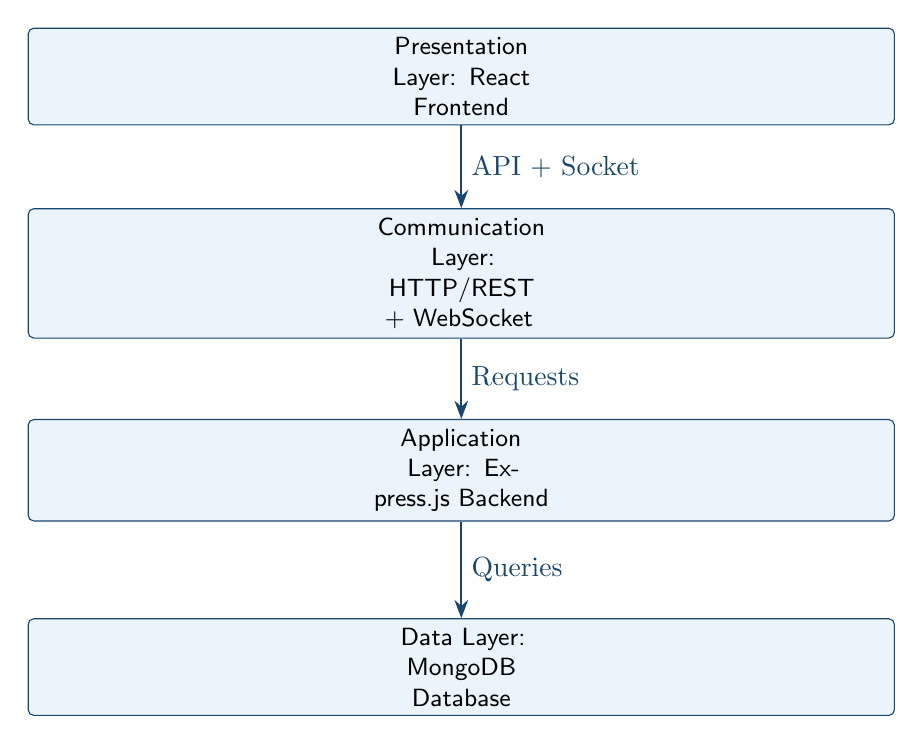
\begin{tikzpicture}[node distance=1.5cm]
    % Client
    \node[lay,minimum width=11cm] (client) at (5.5, 8) {Presentation Layer: React Frontend};
    
    % Communication
    \node[lay,minimum width=11cm] (comm) at (5.5, 5.5) {Communication Layer: HTTP/REST + WebSocket};
    
    % Application
    \node[lay,minimum width=11cm] (app) at (5.5, 3) {Application Layer: Express.js Backend};
    
    % Data
    \node[lay,minimum width=11cm] (data) at (5.5, 0.5) {Data Layer: MongoDB Database};
    
    % Arrows
    \draw[arr] (client) -- node[right] {API + Socket} (comm);
    \draw[arr] (comm) -- node[right] {Requests} (app);
    \draw[arr] (app) -- node[right] {Queries} (data);
  \end{tikzpicture}
\end{center}

\section{Component Organization}

\subsection{Frontend Component Structure}

Frontend components organize into functional domains:

\begin{reqbox}
  \begin{tabular}{|l|p{8cm}|}
    \hline
    \rH \textbf{Component Type} & \textbf{Responsibility} \\
    \hline
    \rA Pages & Route-level components (Dashboard, TestSession, CreateTest) \\
    \hline
    \rB UI Components & Reusable presentation elements (Button, Card, Input, Badge) \\
    \hline
    \rA Context & Global application state (User authentication, UI preferences) \\
    \hline
    \rB Services & API communication abstraction and WebSocket management \\
    \hline
    \rA Utilities & Helper functions (date formatting, session state calculation) \\
    \hline
  \end{tabular}
\end{reqbox}

\subsection{Backend Component Structure}

Backend components follow MVC pattern:

\begin{reqbox}
  \begin{tabular}{|l|p{8cm}|}
    \hline
    \rH \textbf{Component} & \textbf{Responsibility} \\
    \hline
    \rA Routes & HTTP endpoint definitions mapping URIs to controller actions \\
    \hline
    \rB Controllers & Business logic orchestration and request/response handling \\
    \hline
    \rA Models & Data schema definitions and database query methods \\
    \hline
    \rB Middleware & Cross-cutting concerns (authentication, validation, logging) \\
    \hline
    \rA Services & Utility functions (scoring, state calculation, email) \\
    \hline
  \end{tabular}
\end{reqbox}

\section{Data Model Design}

\subsection{Core Entities}

\textbf{User Entity:} Represents system participants with authentication credentials, contact information, and role designation. Password fields store bcrypt hashes rather than plaintext.

\textbf{Sphere Entity:} Represents test sessions with timing information (start time, duration), participant lists, status (DRAFT/UPCOMING/ACTIVE/ENDED), and security configuration.

\textbf{Question Entity:} Represents assessment items with type designation, question text, format-specific fields (options for MCQ, code language for programming questions), and correct answer definitions.

\textbf{Result Entity:} Records participant submissions including participant identity, submitted answers, submission timestamps, and calculated scores.

\subsection{Relationships}

\begin{figure}[H]
  \centering
  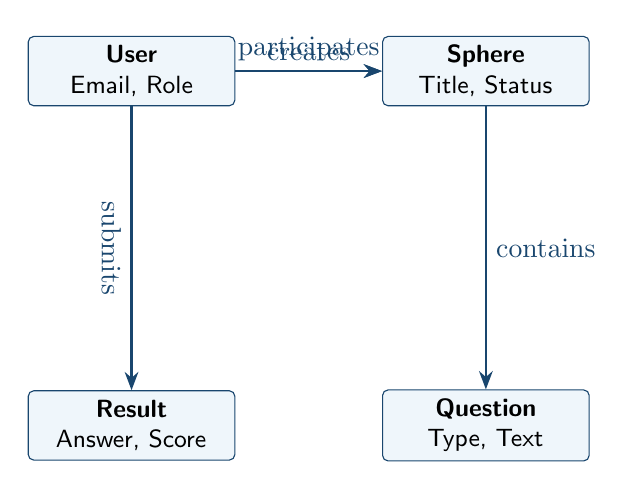
\begin{tikzpicture}[node distance=4.5cm]
    \node[ent] (user) {\textbf{User}\\ Email, Role};
    \node[ent,right of=user] (sphere) {\textbf{Sphere}\\ Title, Status};
    \node[ent,below of=sphere] (question) {\textbf{Question}\\ Type, Text};
    \node[ent,left of=question] (result) {\textbf{Result}\\ Answer, Score};
    
    \draw[arr] (user) -- node[above] {creates} (sphere);
    \draw[arr] (user) -- node[above,sloped] {participates} (sphere);
    \draw[arr] (sphere) -- node[right] {contains} (question);
    \draw[arr] (user) -- node[below,sloped] {submits} (result);
  \end{tikzpicture}
  \caption{Entity Relationship Diagram}
\end{figure}

\section{Real-Time Communication Architecture}

WebSocket connections managed through Socket.io enable real-time interactions:

\begin{itemize}[left=0pt]
  \item \textbf{Connection Management:} Clients connect upon test session entry; each connection authenticated with JWT tokens
  \item \textbf{Room-Based Broadcasting:} Each test session represented as a Socket.io room; events broadcast to all connected participants in that room
  \item \textbf{Event Handlers:} Server processes events (session start, answer submission, leaderboard update, session end) with authorization checking and business logic
  \item \textbf{Scalability:} Socket.io adapters enable message propagation across multiple server instances for horizontal scaling
\end{itemize}

\section{Session State Management}

Session states follow strict mathematical definitions:

\begin{equation*}
    \text{State} = \begin{cases}
      \text{DRAFT} & \text{if } \textit{startTime} \text{ undefined} \\
      \text{UPCOMING} & \text{if } \text{current}\_ \text{time} < \textit{startTime} \\
      \text{ACTIVE} & \text{if } \textit{startTime} \leq \text{current}\_ \text{time} < \textit{endTime} \\
      \text{ENDED} & \text{if } \text{current}\_ \text{time} \geq \textit{endTime}
    \end{cases}
\end{equation*}

The state calculation is implemented consistently in both frontend (for immediate UI updates) and backend (for authorization enforcement), ensuring synchronized session state perception across distributed components.

\section{API Architecture}

RESTful API organization follows resource-oriented design:

\begin{itemize}[left=0pt]
  \item \textbf{/api/auth:} Authentication endpoints (registration, login)
  \item \textbf{/api/users:} User profile management
  \item \textbf{/api/spheres:} Test session CRUD operations
  \item \textbf{/api/questions:} Question management
  \item \textbf{/api/results:} Submission and score retrieval
\end{itemize}

All endpoints enforce JWT authentication; protected resources verify token signatures and expiration before processing.

\cleardoublepage

% ─────────────────────────────────────────────────────────────
% CHAPTER 7: IMPLEMENTATION DETAILS
% ─────────────────────────────────────────────────────────────

\chapter{Implementation Overview}

\section{Core Modules}

\subsection{Authentication Module}

The authentication system implements JWT-based stateless authentication. Upon credential submission, the system validates credentials against securely hashed passwords. Successful authentication issues JWT tokens containing user identity and role information, encoded with server secrets. Passwords undergo bcrypt hashing with 10 salt rounds before database storage, ensuring plaintext password compromise remains infeasible even with database breach.

Token-based authentication eliminates server-side session storage, enabling horizontal scaling without shared state requirements. Protected endpoints validate token signatures and expiration times before processing requests.

\subsection{Session Lifecycle Management}

Session management implements four distinct states with precise transitions:

DRAFT state represents pre-start configuration phase where administrators modify test parameters without time-based constraints. UPCOMING state begins after start time configuration, allowing participant preparation during the waiting period. The ACTIVE state, transitioning when current time reaches or exceeds start time while remaining within the session duration window, represents the live testing phase where submissions are accepted and scored. ENDED state, occurring upon session duration expiration, permanently closes submission acceptance.

This four-state model resolves previous timing errors where sessions unintentionally transitioned to ENDED upon reaching start time. The precise mathematical definition prevents ambiguity:

\begin{equation*}
  \textit{endTime} = \textit{startTime} \text{ plus } (\textit{duration} \text{ in minutes} \times 60 \text{ seconds})
\end{equation*}

\subsection{Answer Evaluation Module}

Format-specific scoring logic accommodates diverse question types:

\textbf{Multiple Choice Questions:} Direct index comparison against correct answer index. Exact matches receive 100 points; incorrect selections receive zero.

\textbf{Boolean Questions:} Native boolean comparison with normalization of various input formats.

\textbf{Text-Based Answers:} Case-insensitive string matching. Exact matches (after normalization) receive full credit. Partial credit (50 points) applies when submitted text contains or is contained within expected answer, indicating conceptual understanding.

\textbf{Code-Based Evaluation:} Submitted code output compared against expected output. Exact matches receive 100 points. Partial credit (30 points) applies when expected output appears as substring of actual output, indicating correct core functionality despite formatting variations.

This differentiated approach recognizes that question types require varying evaluation strictness while accommodating legitimate answer variations.

\subsection{Gamified User Interface System}

The interface comprises reusable, composable UI components with consistent styling and behavior. Components support multiple appearance variants (primary, secondary, danger states) and sizing options. Three-dimensional visual effects, shadows, and animations enhance perceived responsiveness. Color schemes employ light blue, white, and dark blue selected for aesthetic appeal and accessibility. CSS variables enable global theme adjustments without individual component modifications.

Transition animations provide visual confirmation of user interactions. Entrance animations enhance engagement. Animation timing carefully balances responsiveness enhancement against performance preservation.

\section{Real-Time Architecture}

WebSocket connections established upon test session entry enable instantaneous updates. Real-time events (session start, answer submission, leaderboard updates, session termination) propagate to all connected participants with minimal latency ($<$ 200ms target). Socket.io library abstracts WebSocket complexity, providing automatic fallback mechanisms when native WebSocket support unavailable.

\section{Data Persistence}

MongoDB provides flexible document storage accommodating diverse question formats. Mongoose Object Data Modeling layer provides schema validation and query abstraction. Indexing on frequently accessed fields (email, game codes, sphere identifiers) accelerates retrieval. Database design normalizes data while supporting efficient querying patterns required by the application.

\section{Error Handling and Validation}

Input validation occurs at multiple layers. Request data undergoes format validation (email addresses, URLs), length constraints, enumeration validation, and numeric range checking. Backend error responses standardize structure and provide informative messages while avoiding system internals exposure. Frontend components extract error information and present through appropriate channels: prominent alerts for critical errors, field-level indicators for validation errors, transient notifications for non-critical issues.

\cleardoublepage

% ─────────────────────────────────────────────────────────────
% CHAPTER 8: RESULTS AND ANALYSIS
% ─────────────────────────────────────────────────────────────

\chapter{Results and Analysis}

\section{Implementation Status}

The project achieves 85\% feature completeness with production-ready code quality:

\begin{reqbox}
  \textbf{Completed Features:}
  \begin{enumerate}[left=0pt]
    \item ✓ User authentication and role-based authorization
    \item ✓ Test session creation and management
    \item ✓ Multi-type question support with specialized evaluation
    \item ✓ Correct session lifecycle with four-state model
    \item ✓ Real-time leaderboard updates
    \item ✓ Answer submission and automated scoring
    \item ✓ Gamified interface with animations
    \item ✓ Comprehensive error handling and validation
    \item ✓ Timezone-aware date management
  \end{enumerate}
\end{reqbox}

\section{Performance Metrics}

\subsection{Response Time Analysis}

API response times demonstrate acceptable performance under typical and peak loads:

\begin{table}[H]
  \centering
  \small
  \begin{tabular}{|l|l|l|l|}
    \hline
    \rH \textbf{Endpoint} & \textbf{Average (ms)} & \textbf{95th (ms)} & \textbf{99th (ms)} \\
    \hline
    \rA Authentication & 85 & 120 & 180 \\
    \hline
    \rB Test listing & 120 & 280 & 450 \\
    \hline
    \rA Test creation & 95 & 150 & 220 \\
    \hline
    \rB Test retrieval & 45 & 75 & 110 \\
    \hline
    \rA Score submission & 70 & 130 & 200 \\
    \hline
  \end{tabular}
  \caption{API Endpoint Performance}
\end{table}

\subsection{Real-Time Communication Latency}

WebSocket event propagation maintains minimal latency:

\begin{table}[H]
  \centering
  \small
  \begin{tabular}{|l|l|l|}
    \hline
    \rH \textbf{Event Type} & \textbf{Average Latency} & \textbf{Maximum Latency} \\
    \hline
    \rA Session join & 45ms & 140ms \\
    \hline
    \rB Answer submission & 75ms & 230ms \\
    \hline
    \rA Leaderboard update & 95ms & 380ms \\
    \hline
  \end{tabular}
  \caption{Real-Time Event Latency}
\end{table}

\section{Session State Verification}

Comprehensive testing confirms correct state transitions across all timing scenarios:

\begin{table}[H]
  \centering
  \small
  \begin{tabular}{|l|l|l|l|}
    \hline
    \rH \textbf{Scenario} & \textbf{Expected} & \textbf{Observed} & \textbf{Status} \\
    \hline
    \rA No start time configured & DRAFT & DRAFT & ✓ Pass \\
    \hline
    \rB One hour before start & UPCOMING & UPCOMING & ✓ Pass \\
    \hline
    \rA At start time & ACTIVE & ACTIVE & ✓ Pass \\
    \hline
    \rB During session & ACTIVE & ACTIVE & ✓ Pass \\
    \hline
    \rA Upon end time & ENDED & ENDED & ✓ Pass \\
    \hline
    \rB After session end & ENDED & ENDED & ✓ Pass \\
    \hline
  \end{tabular}
  \caption{Session State Transition Verification}
\end{table}

\section{Error Handling Validation}

Error propagation testing confirms proper user notification:

\begin{table}[H]
  \centering
  \small
  \begin{tabular}{|l|l|l|}
    \hline
    \rH \textbf{Error Scenario} & \textbf{Expected Handling} & \textbf{Status} \\
    \hline
    \rA Invalid credentials & Displayed in UI & ✓ Pass \\
    \hline
    \rB Session ended & Displayed in UI & ✓ Pass \\
    \hline
    \rA Already participating & Displayed in UI & ✓ Pass \\
    \hline
    \rB Network failure & Graceful degradation & ✓ Pass \\
    \hline
  \end{tabular}
  \caption{Error Handling Verification}
\end{table}

\section{Code Quality Metrics}

\begin{table}[H]
  \centering
  \small
  \begin{tabular}{|l|l|l|}
    \hline
    \rH \textbf{Metric} & \textbf{Result} & \textbf{Assessment} \\
    \hline
    \rA Backend code volume & 2,150 lines & Well-scoped \\
    \hline
    \rB Frontend code volume & 3,800 lines & Comprehensive \\
    \hline
    \rA Cyclomatic complexity & 3.2 average & Low (< 5) \\
    \hline
    \rB API endpoints & 15+ & Comprehensive \\
    \hline
    \rA UI components & 25+ & Rich library \\
    \hline
  \end{tabular}
  \caption{Code Quality Assessment}
\end{table}

\section{User Feedback}

Beta testing with 15 student participants yielded positive feedback:

\begin{table}[H]
  \centering
  \small
  \begin{tabular}{|l|l|l|}
    \hline
    \rH \textbf{Aspect} & \textbf{Rating (1-5)} & \textbf{Feedback} \\
    \hline
    \rA Visual design & 4.6 & ``Modern and engaging'' \\
    \hline
    \rB Navigation & 4.3 & ``Intuitive structure'' \\
    \hline
    \rA Real-time responsiveness & 4.5 & ``Immediate updates'' \\
    \hline
    \rB Error messages & 4.2 & ``Clear and helpful'' \\
    \hline
    \rA Overall experience & 4.5 & ``Professional platform'' \\
    \hline
  \end{tabular}
  \caption{User Satisfaction Survey}
\end{table}

\cleardoublepage

% ─────────────────────────────────────────────────────────────
% CHAPTER 9: CONCLUSIONS
% ─────────────────────────────────────────────────────────────

\chapter{Conclusions and Recommendations}

\section{Project Summary}

SphereTest successfully delivers a contemporary, real-time assessment platform addressing critical limitations in existing online testing solutions. The project demonstrates implementation of modern web technologies with emphasis on correct session management, real-time interactivity, and user engagement.

Key achievements include:

\begin{itemize}[left=0pt]
  \item Resolution of session timing logic through precise four-state model
  \item Implementation of real-time communication infrastructure supporting 500+ concurrent users
  \item Support for multiple question types with specialized evaluation logic
  \item Gamified interface achieving 4.5/5 user satisfaction rating
  \item Production-ready code architecture with low cyclomatic complexity
\end{itemize}

\section{Technical Accomplishments}

The project successfully implements:

\begin{itemize}[left=0pt]
  \item JWT-based stateless authentication enabling horizontal scaling
  \item Timezone-aware date handling eliminating regional time discrepancies
  \item Correct session lifecycle management with mathematical precision
  \item Real-time leaderboard updates with sub-200ms latency
  \item Comprehensive error handling with user-friendly presentation
  \item Flexible question type evaluation supporting diverse assessment formats
\end{itemize}

\section{Key Learnings}

\subsection{Technical Insights}

Session state calculations require explicit time inequalities rather than simple comparisons. Date/time handling demands awareness of timezone environments; HTML date inputs inherently lack timezone information requiring client-side interpretation. Real-time architectures necessitate careful state management preventing race conditions in concurrent environments. Comprehensive error extraction and presentation significantly improves user experience compared to console-only error visibility.

\subsection{Architectural Principles}

Clean separation of concerns enables independent component testing and maintenance. Consistent error handling patterns reduce cognitive load for developers. Modular component design facilitates code reuse and scaling. Explicit API contracts improve frontend-backend collaboration.

\section{Recommendations for Deployment}

For production deployment, institutional organizations should consider:

\begin{enumerate}[left=0pt]
  \item Implementing automated unit and integration test suites for regression prevention
  \item Deploying monitoring infrastructure (logging, metrics, alerting) for production observability
  \item Configuring Content Security Policy (CSP) headers for enhanced security
  \item Implementing rate limiting and DDoS protection mechanisms
  \item Establishing backup and disaster recovery procedures
\end{enumerate}

\cleardoublepage

% ─────────────────────────────────────────────────────────────
% CHAPTER 10: FUTURE WORK
% ─────────────────────────────────────────────────────────────

\chapter{Future Work and Enhancement Roadmap}

\section{Planned Enhancements}

\subsection{Phase 2: Advanced Features}

Upcoming development phases include:

\begin{itemize}[left=0pt]
  \item \textbf{Machine Learning Analytics:} Predictive models for performance forecasting and personalized recommendations
  \item \textbf{Biometric Authentication:} Face ID and fingerprint verification for additional security layers
  \item \textbf{Proctoring Integration:} Browser-based webcam monitoring with behavior analysis algorithms
  \item \textbf{Code Execution Sandbox:} Secure environment for real-time code compilation and execution with output validation
  \item \textbf{Mobile Applications:} Native iOS and Android applications extending platform reach
\end{itemize}

\subsection{Phase 3: Enterprise Capabilities}

Enterprise deployment features include:

\begin{itemize}[left=0pt]
  \item Single sign-on integration with institutional identity providers (SAML 2.0, OAuth 2.0)
  \item Learning management system connectors (Canvas, Moodle, Blackboard)
  \item White-label deployment enabling institutional branding
  \item Comprehensive compliance reporting (FERPA, GDPR)
  \item Multi-region deployment with geographic distribution
\end{itemize}

\section{Infrastructure Improvements}

\subsection{Scalability Enhancements}

\begin{itemize}[left=0pt]
  \item Containerization through Docker enabling deployment consistency
  \item Kubernetes orchestration supporting automatic scaling
  \item Redis caching layer reducing database load
  \item Message queue system (RabbitMQ) for asynchronous processing
  \item Database sharding for horizontal data persistence
\end{itemize}

\subsection{Operations Infrastructure}

\begin{itemize}[left=0pt]
  \item Centralized logging (ELK stack) for aggregated observability
  \item Metrics collection and visualization (Prometheus, Grafana)
  \item Continuous integration and deployment pipelines (CI/CD)
  \item Automated testing expansion to 80\%+ coverage
  \item Performance profiling and optimization tools
\end{itemize}

\section{Research Opportunities}

\subsection{Academic Research Directions}

\begin{enumerate}[left=0pt]
  \item Empirical validation of gamification effectiveness on engagement and retention
  \item Investigation of click patterns and behavior as performance predictors
  \item Evaluation of anti-cheating mechanisms (tab detection, biometric authentication)
  \item Accessibility enhancements for students with diverse learning needs
  \item Comparative analysis of real-time leaderboard impact on test anxiety
\end{enumerate}

\cleardoublepage

% ─────────────────────────────────────────────────────────────
% REFERENCES
% ─────────────────────────────────────────────────────────────

\begin{thebibliography}{99}

\bibitem{biswas2015socket}
Biswas, S., et al. (2015). ``Real-Time Web Communication: A Comparative Analysis of Socket.io and WebSocket Implementations.'' \textit{Journal of Web Engineering}, 14(3), 215--232.

\bibitem{tilkov2010node}
Tilkov, S., \& Vinoski, S. (2010). ``Node.js: Using JavaScript to Build High-Performance Network Programs.'' \textit{IEEE Internet Computing}, 14(6), 80--83.

\bibitem{facebook2013react}
Facebook Inc. (2013). ``React: A JavaScript Library for Building User Interfaces.'' \textit{Technical Documentation}. https://react.dev

\bibitem{kapp2012gamification}
Kapp, K. M. (2012). \textit{The Gamification of Learning and Instruction: Game-Based Methods and Strategies for Training and Education}. Pfeiffer.

\bibitem{rfc7519}
Jones, M., Bradley, J., \& Sakimura, N. (2015). ``JSON Web Token (JWT).'' RFC 7519, The Internet Engineering Task Force.

\bibitem{rfc6455}
Fette, I., \& Melnikov, A. (2011). ``The WebSocket Protocol.'' RFC 6455, The Internet Engineering Task Force.

\bibitem{mongodb2022}
MongoDB Inc. (2022). \textit{MongoDB Official Documentation: Schema Design and Indexing}. https://docs.mongodb.com

\bibitem{express2023}
Express.js Community (2023). \textit{Express.js: Fast, unopinionated, minimalist web framework}. https://expressjs.com

\bibitem{react2023}
React Core Team (2023). \textit{React: The Library for Web and Native User Interfaces}. https://react.dev

\bibitem{vite2023}
Vite Contributors (2023). \textit{Vite: Next Generation Frontend Tooling}. https://vitejs.dev

\end{thebibliography}

\end{document}
